\begin{highlightblock}[Combinatorial Circuit]
Write an entity and architecture for the system described in Figure \ref{fig:comb}. This entity has two inputs (\vhdl{operand_a_i} and \vhdl{operand_b_i}) and two outputs. The first output \vhdl{and_o} should be calculated as the logical AND operation of the two inputs and the second output \vhdl{or_o} should be calculated as the logical OR operation of the two inputs.

\begin{center}
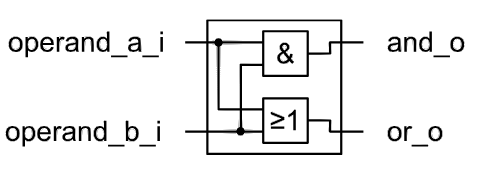
\includegraphics[width=0.5\linewidth]{images/combinatorial-circuit.png}

Figure \refstepcounter{figure}\arabic{figure}: Combinatorial Circuit\label{fig:comb}
\end{center}

\textbf{To-Do-List}

\begin{itemize}
\item  Write the entity and architecture of the system in VHDL. Use one .vhd file for the entity and one .vhd file for the architecture.
\item Write a testbench in VHDL (extra file). Simulate the system using Modelsim and put the screenshots showing the output of the waveform window in the report pdf.
\item Discuss the results of the simulation in a few sentences.
\end{itemize}

\end{highlightblock}
